%% !TEX root = manual.tex

\chapter{Introduction}
\label{sec:intro}

\section{Overview}
\label{sec:intro:overview}

The \sstmacro software package provides a simulator for large-scale parallel computer architectures. 
It permits the coarse-grained study of distributed-memory applications. 
The simulator is driven from either a trace file or skeleton application. 
The simulator architecture is modular, allowing it to easily be extended with additional network models, 
trace file formats, software services, and processor models.

Simulation can be broadly categorized as either off-line or on-line.
Off-line simulators typically first run a full parallel application on a real machine,
recording certain communication and computation events to a simulation trace.
This event trace can then be replayed post-mortem in the simulator.
Most common are MPI traces which record all MPI events, and
\sstmacro provides the DUMPI utility (\ref{sec:tutorial:dumpi}) for collecting and replaying MPI traces. 
Trace extrapolation can extend the usefulness of off-line simulation by estimating large or untraceable system scales without   
having to collect a trace, but it is limited.

We turn to on-line simulation when the hardware or applications parameters need to change.
On-line simulators instead run real application code, allowing native C/C++/Fortran to be compiled directly into the simulator.
\sstmacro intercepts certain function calls, estimating how much time passes rather than actually executing the function.
In MPI programs, for example, calls to MPI\_Send are linked to the simulator instead of passing to the real MPI library.
If desired, \sstmacro can actually be a full MPI \emph{emulator}, delivering messages between ranks and replicating the behavior of a full MPI implementation.

Although \sstmacro supports both on-line and off-line modes, on-line simulation is encouraged because
event traces are much less flexible, containing a fixed sequence of events.
Application inputs and number of nodes cannot be changed. 
Without a flexible control flow, it also cannot simulate dynamic behavior like load balancing or faults.
On-line simulation can explore a much broader problem space since they evolve directly in the simulator.

For large, system-level experiments with thousands of network endpoints, high-accuracy cycle-accurate simulation is not possible,
or at least not convenient.
Simulation requires coarse-grained approximations to be practical.
\sstmacro is therefore designed for specific cost/accuracy tradeoffs.
It should still capture complex cause/effect behavior in applications and hardware, but be efficient enough to simulate at the system-level. 
For speeding up simulator execution, we encourage \textit{skeletonization}, discussed further in Chapter \ref{chap:appsAndSkeletonization}. 
A high-quality skeleton is an application model that reproduces certain characteristics with only limited computation.  
We also encourage uncertainty quantification (UQ) for validating simulator results.
Skeletonization and UQ are the two main elements in the ``canonical'' \sstmacro workflow (Figure \ref{fig:workflow}).

\begin{figure}[t]
  \centering
    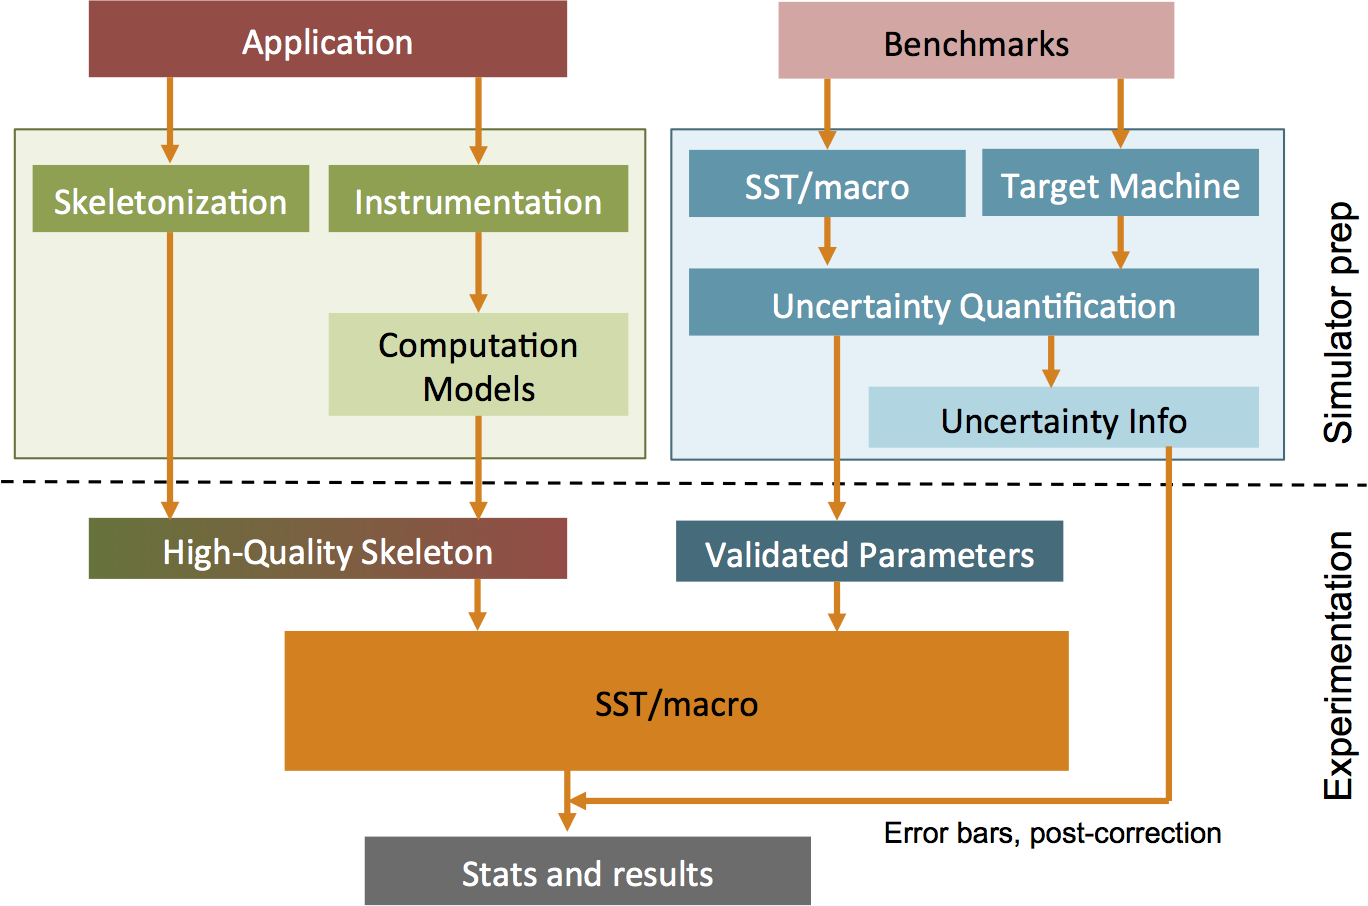
\includegraphics[width=0.99\columnwidth]{figures/workflow.png}
      \caption{SST/macro workflow.}
      \label{fig:workflow}
\end{figure}

Because of its popularity, MPI is one of our main priorities in providing programming model support.  
Some MPI-3 functions and MPI one-sided functions are not implemented.
This will lead to compile errors with an obvious ``not implement'' compiler message.

\section{Preview of Things to Come}
Suppose you have the basic MPI application below that executes a simple send/recv operation.
One could use \inlineshell{mpicc} or \inlineshell{mpic++} to compile and run as an actual MPI program.
This requires spawning all the processes and running them in parallel.
Suppose, however, you wanted to simulate an entire MPI job launch within a single process.
This might prove very useful for debugging since you could just run GDB or Valgrind on a single process.
It might take a while, but for small runs (16 ranks or so) you could debug right on your laptop the same you do for a serial program.

\begin{CppCode}
int size = atoi(argv[1]);
if (rank == 0){
 int partner = 1;
  MPI_Send(buffer, size, MPI_INT, partner, tag, MPI_COMM_WORLD);
} else {
  int partner = 0;
  MPI_Recv(buffer, size, MPI_INT, partner, tag, MPI_COMM_WORLD, MPI_STATUS_IGNORE);
}
MPI_Barrier(MPI_COMM_WORLD);

if (rank == 0){
  printf("Rank 0 finished at t=%8.4f ms\n", MPI_Wtime()*1e3);
}
\end{CppCode}

This is exactly the functionality that SST/macro provides.
Instead of using \inlineshell{mpic++}, you compile the code with {sst++}.
This modifies your code and intercepts MPI calls, running them through the simulator instead of an actual MPI implementation.
Your code will execute and run exactly the same, and your application won't even know the difference.
You now need a parameter file with information like:

\begin{ViFile}
node {
 app1 {
  name = send_recv
  launch_cmd = aprun -n 2
  argv = 20
 }
}
\end{ViFile}
Rather than launching your code using \inlineshell{mpirun} or similar, you put all your command line parameters into a \inlineshell{parameters.ini} file and run:

\begin{ShellCmd}
shell> sstmac -f parameters.ini
\end{ShellCmd}
The simulator then executes your application exactly as if you had been a real system and run:

\begin{ShellCmd}
shell> aprun -n 2 ./send_recv 20
\end{ShellCmd}
Things get more complicated when you bring skeletonization into play.
The use case above is \emph{emulation}, exactly reproducing MPI functionality.
In \emph{skeletonization} or \emph{simulation}, SST/macro will mimic as closely as possible the original application,
but avoids as much computation and as much memory allocation as possible.
This allows packing in as many simulated (virtual) MPI ranks as possible into your single \inlineshell{sstmac} process.

\section{What To Expect In The User's Manual}
This user's manual is mainly designed for those who wish to perform experiments with \emph{new} applications using \emph{existing} hardware models.
This has been the dominant use case and we therefore classify those doing application experiments as ``users'' and those making new hardware models ``developers.''
Getting applications to run in SST/macro should be very straightforward and requires no knowledge of simulator internal code.
Making new hardware models is much more in depth and requires learning some basics of core simulator code.
Those interested in making new hardware models should consult the developer's manual in the top-level source directory.
